%----------
%   IMPORTANTE
%----------

% Si nunca has utilizado LaTeX es conveniente que aprendas una serie de conceptos básicos antes de utilizar esta plantilla. Te aconsejamos que leas previamente algún tutorial (puedes encontar muchos en Internet).

% Esta plantilla está basada en las recomendaciones de la guía "Trabajo fin de Grado: Escribir el TFG", que encontrarás en http://uc3m.libguides.com/TFG/escribir
% contiene recomendaciones de la Biblioteca basadas principalmente en estilos APA e IEEE, pero debes seguir siempre las orientaciones de tu Tutor de TFG y la normativa de TFG para tu titulación.

% Encontrarás un ejemplo de TFG realizado con esta misma plantilla en la carpeta "_ejemplo_TFG_2019". Consúltalo porque contiene ejemplos útiles para incorporar tablas, figuras, listados de código, bibliografía, etc.


%----------
%	CONFIGURACIÓN DEL DOCUMENTO
%----------

% Definimos las características del documento y añadimos una serie de paquetes (\usepackage{package}) que agregan funcionalidades a LaTeX.

\documentclass[12pt]{report} %fuente a 12pt

\usepackage{lipsum} % el paquete lipsum permite rellenar texto del tipo "Lorem ipsum" a modo de ejemplo

% MÁRGENES: 2,5 cm sup. e inf.; 3 cm izdo. y dcho.
\usepackage[
a4paper,
vmargin=2.5cm,
hmargin=3cm
]{geometry}

% INTERLINEADO: Estrecho (6 ptos./interlineado 1,15) o Moderado (6 ptos./interlineado 1,5)
\renewcommand{\baselinestretch}{1.15}
\parskip=6pt

% DEFINICIÓN DE COLORES para portada y listados de código
\usepackage[table]{xcolor}
\definecolor{azulUC3M}{RGB}{0,0,102}
\definecolor{gray97}{gray}{.97}
\definecolor{gray75}{gray}{.75}
\definecolor{gray45}{gray}{.45}

% Soporte para GENERAR PDF/A --es importante de cara a su inclusión en e-Archivo porque es el formato óptimo de preservación y a la generación de metadatos, tal y como se describe en http://uc3m.libguides.com/ld.php?content_id=31389625. En la carpeta incluímos el archivo plantilla_tfg_2017.xmpdata en el que puedes incluir los metadatos que se incorporarán al archivo PDF cuando lo compiles. Ese archivo debe llamarse igual que tu archivo .tex. Puedes ver un ejemplo en esta misma carpeta.
\usepackage[a-1b]{pdfx}

% ENLACES
\usepackage{hyperref}
\hypersetup{colorlinks=true,
	linkcolor=black, % enlaces a partes del documento (p.e. índice) en color negro
	urlcolor=blue} % enlaces a recursos fuera del documento en azul

% EXPRESIONES MATEMATICAS
\usepackage{amsmath,amssymb,amsfonts,amsthm}

\usepackage{txfonts} 
\usepackage[T1]{fontenc}
\usepackage[utf8]{inputenc}

\usepackage[english]{babel} 
\usepackage[babel, english=american]{csquotes}
\AtBeginEnvironment{quote}{\small}

% diseño de PIE DE PÁGINA
\usepackage{fancyhdr}
\pagestyle{fancy}
\fancyhf{}
\renewcommand{\headrulewidth}{0pt}
\rfoot{\thepage}
\fancypagestyle{plain}{\pagestyle{fancy}}

% DISEÑO DE LOS TÍTULOS de las partes del trabajo (capítulos y epígrafes o subcapítulos)
\usepackage{titlesec}
\usepackage{titletoc}
\titleformat{\chapter}[block]
{\large\bfseries\filcenter}
{\thechapter.}
{5pt}
{\MakeUppercase}
{}
\titlespacing{\chapter}{0pt}{0pt}{*3}
\titlecontents{chapter}
[0pt]                                               
{}
{\contentsmargin{0pt}\thecontentslabel.\enspace\uppercase}
{\contentsmargin{0pt}\uppercase}                        
{\titlerule*[.7pc]{.}\contentspage}                 

\titleformat{\section}
{\bfseries}
{\thesection.}
{5pt}
{}
\titlecontents{section}
[5pt]                                               
{}
{\contentsmargin{0pt}\thecontentslabel.\enspace}
{\contentsmargin{0pt}}
{\titlerule*[.7pc]{.}\contentspage}

\titleformat{\subsection}
{\normalsize\bfseries}
{\thesubsection.}
{5pt}
{}
\titlecontents{subsection}
[10pt]                                               
{}
{\contentsmargin{0pt}                          
	\thecontentslabel.\enspace}
{\contentsmargin{0pt}}                        
{\titlerule*[.7pc]{.}\contentspage}  


% DISEÑO DE TABLAS. Puedes elegir entre el estilo para ingeniería o para ciencias sociales y humanidades. Por defecto, está activado el estilo de ingeniería. Si deseas utilizar el otro, comenta las líneas del diseño de ingeniería y descomenta las del diseño de ciencias sociales y humanidades
\usepackage{multirow} %permite combinar celdas 
\usepackage{caption} %para personalizar el título de tablas y figuras
\usepackage{floatrow} %utilizamos este paquete y sus macros \ttabbox y \ffigbox para alinear los nombres de tablas y figuras de acuerdo con el estilo definido. Para su uso ver archivo de ejemplo 
\usepackage{array} % con este paquete podemos definir en la siguiente línea un nuevo tipo de columna para tablas: ancho personalizado y contenido centrado
\newcolumntype{P}[1]{>{\centering\arraybackslash}p{#1}}
\DeclareCaptionFormat{upper}{#1#2\uppercase{#3}\par}

% Diseño de tabla para ingeniería
\captionsetup[table]{
	format=upper,
	justification=centering,
	labelsep=period,
	width=.75\linewidth,
	labelfont=small,
	font=small,
}

%Diseño de tabla para ciencias sociales y humanidades
%\captionsetup[table]{
%	justification=raggedright,
%	labelsep=period,
%	labelfont=small,
%	singlelinecheck=false,
%	font={small,bf}
%}


% DISEÑO DE FIGURAS. Puedes elegir entre el estilo para ingeniería o para ciencias sociales y humanidades. Por defecto, está activado el estilo de ingeniería. Si deseas utilizar el otro, comenta las líneas del diseño de ingeniería y descomenta las del diseño de ciencias sociales y humanidades
\usepackage{graphicx}
\graphicspath{{imagenes/}} %ruta a la carpeta de imágenes

% Diseño de figuras para ingeniería
\captionsetup[figure]{
	format=hang,
	name=Fig.,
	singlelinecheck=off,
	labelsep=period,
	labelfont=small,
	font=small		
}

% Diseño de figuras para ciencias sociales y humanidades
%\captionsetup[figure]{
%	format=hang,
%	name=Figure,
%	singlelinecheck=off,
%	labelsep=period,
%	labelfont=small,
%	font=small		
%}


% NOTAS A PIE DE PÁGINA
\usepackage{chngcntr} %para numeración contínua de las notas al pie
\counterwithout{footnote}{chapter}

% LISTADOS DE CÓDIGO
% soporte y estilo para listados de código. Más información en https://es.wikibooks.org/wiki/Manual_de_LaTeX/Listados_de_código/Listados_con_listings
\usepackage{listings}

% definimos un estilo de listings
\lstdefinestyle{estilo}{ frame=Ltb,
	framerule=0pt,
	aboveskip=0.5cm,
	framextopmargin=3pt,
	framexbottommargin=3pt,
	framexleftmargin=0.4cm,
	framesep=0pt,
	rulesep=.4pt,
	backgroundcolor=\color{gray97},
	rulesepcolor=\color{black},
	%
	basicstyle=\ttfamily\footnotesize,
	keywordstyle=\bfseries,
	stringstyle=\ttfamily,
	showstringspaces = false,
	commentstyle=\color{gray45},     
	%
	numbers=left,
	numbersep=15pt,
	numberstyle=\tiny,
	numberfirstline = false,
	breaklines=true,
	xleftmargin=\parindent
}

\captionsetup[lstlisting]{font=small, labelsep=period}
% fijamos el estilo a utilizar 
\lstset{style=estilo}
\renewcommand{\lstlistingname}{\uppercase{Código}}


%BIBLIOGRAFÍA - PUEDES ELEGIR ENTRE ESTILO IEEE O APA. POR DEFECTO ESTÁ CONFIGURADO IEEE. SI DESEAS USAR APA, COMENTA LAS LÍNEA DE IEEE Y DESCOMENTA LAS DE APA. Si haces cambios en la configuración de la bibliografía y no obtienes los resultados esperados, es recomendable limpiar los archivos auxiliares y volver a compilar en este orden: COMPILAR-BIBLIOGRAFIA-COMPILAR
% Tienes más información sobre cómo generar bibliografía en http://tex.stackexchange.com/questions/154751/biblatex-with-biber-configuring-my-editor-to-avoid-undefined-citations , https://es.sharelatex.com/learn/Bibliography_management_in_LaTeX y en http://www.ctan.org/tex-archive/macros/latex/exptl/biblatex-contrib
% También te recomendamos consultar la guía temática de la Biblioteca sobre citas bibliográficas: http://uc3m.libguides.com/guias_tematicas/citas_bibliograficas/inicio

% CONFIGURACIÓN PARA LA BIBLIOGRAFÍA IEEE
\usepackage[backend=biber, style=ieee, isbn=false,sortcites, maxbibnames=5, minbibnames=1]{biblatex} % Configuración para el estilo de citas de IEEE, recomendado para el área de ingeniería. "maxbibnames" indica que a partir de 5 autores trunque la lista el primero (minbibnames) y añada "et al." tal y como se utiliza en el estilo IEEE.

%CONFIGURACIÓN PARA LA BIBLIOGRAFÍA APA
%\usepackage[style=apa, backend=biber, natbib=true, hyperref=true, uniquelist=false, sortcites]{biblatex}
%\DeclareLanguageMapping{spanish}{spanish-apa}

\addbibresource{bibliografia/bibliografia.bib} % llama al archivo bibliografia.bib que utilizamos de ejemplo


%-------------
%	DOCUMENTO
%-------------

\begin{document}
	\pagenumbering{roman}
	
	%----------
	%	PORTADA
	%----------	
	\begin{titlepage}
		\begin{sffamily}
			\color{azulUC3M}
			\begin{center}
				\begin{figure}[H] %incluimos el logotipo de la Universidad
					\makebox[\textwidth][c]{
\includegraphics[width=16cm]{Portada_Logo.png}}
				\end{figure}
				\vspace{2.5cm}
				\begin{Large}
					University Degree in Energy Engineering\\			
					2016-2017\\
					\vspace{2cm}		
					\textsl{Bachelor Thesis}
					\bigskip
					
				\end{Large}
				{\Huge ``Design of a Bachelor Thesis in \LaTeX''}\\
				\vspace*{0.5cm}
				\rule{10.5cm}{0.1mm}\\
				\vspace*{0.9cm}
				{\LARGE Carlos Tercero Tercero}\\ 
				\vspace*{1cm}
				\begin{Large}
					Juan Profesor Profesor\\
					Leganés, 2017\\
				\end{Large}
			\end{center}
			\vfill
			\color{black}
			
\includegraphics[width=4.2cm]{imagenes/creativecommons.png}\\
			%\emph{[Include this code in case you want your Bachelor Thesis published in Open Access University Repository]}\\
			This work is licensed under Creative Commons \textbf{Attribution – Non Commercial – Non Derivatives}
		\end{sffamily}
	\end{titlepage}

\newpage %página en blanco o de cortesía
\thispagestyle{empty}
\mbox{}

%----------
%	RESUMEN Y PALABRAS CLAVE
%----------	
\renewcommand\abstractname{\large\uppercase{Summary}}
\begin{abstract}
\thispagestyle{plain}
\setcounter{page}{3}
	
	\lipsum[1-3]
	
	\textbf{Keywords:}
	Intellectual work; Scientific investigation; Writing; Styling
	
	\vfill
\end{abstract}
	\newpage %página en blanco o de cortesía
	\thispagestyle{empty}
	\mbox{}


%----------
%	DEDICATORIA
%----------	
\chapter*{Dedication}

\setcounter{page}{5}
	
	\lipsum [4-5]	
		
	\vfill
	
	\newpage %página en blanco o de cortesía
	\thispagestyle{empty}
	\mbox{}
	

%----------
%	ÍNDICES
%----------	

%--
%Índice general
%-
\tableofcontents
\thispagestyle{fancy}

\newpage %página en blanco o de cortesía
\thispagestyle{empty}
\mbox{}

%--
%Índice de figuras. Si no se incluyen, comenta las líneas siguientes
%-
\listoffigures
\thispagestyle{fancy}

\newpage %página en blanco o de cortesía
\thispagestyle{empty}
\mbox{}

%--
%Índice de tablas. Si no se incluyen, comenta las líneas siguientes
%-
\listoftables
\thispagestyle{fancy}

\newpage %página en blanco o de cortesía
\thispagestyle{empty}
\mbox{}


%----------
%	TRABAJO
%----------	
\clearpage
\pagenumbering{arabic} % numeración con múmeros arábigos para el resto de la publicación	

\chapter{Introduction}

\section{Motivation of Work}
\lipsum[1-3]

\section{Goals}
\lipsum[1-2]

\section{Regulatory framework}
\lipsum[5-6]


\chapter{Status of the Question}

\section{Current situation}
\lipsum[10-13]

\section{Current framework}
\lipsum[8-9]

\section{Design of solutions}
\lipsum[4-5]


\chapter{Analysis of the situation}

\section{Description}
\lipsum[19]
\begin{figure}[H]
	\ffigbox[\FBwidth]
	{\caption[The conjoined triangle of success]{The conjoined triangle of success \cite{kruger}}} % [Aquí ponemos como queremos que aparezca en el índice, sin la referencia]{Aquí como queremos que aparezca en el documento, con la referencia}
	{
\includegraphics[scale=0.6]{success.jpg}}
\end{figure}

\lipsum[9-10]

\blockquote{Entre los principales objetivos de la Declaración de Bolonia se encuentra la armonización de los sistemas nacionales de titulaciones basado, esencialmente, en los dos ciclos principales de grado y postgrado, así como	el establecimiento de un sistema de créditos europeos como el sistema ECTS y la implantación de un suplemento europeo a los títulos emitidos por las instituciones educativas de  enseñanza  superior. (Real  Decreto  1044/2003,  de  1  de  agosto,  por  el  que  se  establece  el  procedimiento para la expedición por las universidades del Suplemento Europeo al Titulo. Boletín Oficial del Estado (11 de septiembre de 2003), págs. 33848-33853)}

\lipsum[20-22]

\section{Requirements}

\lipsum[15]

\subsection{First level}
\lipsum[15-16]

\begin{equation} % Si queremos que la expresión vaya numerada hay que escribirla entre \begin y \end {equation}.
\log \mu_{ijk}= \lambda + \lambda_i ^I + \lambda_j ^J+\lambda_k ^K+\lambda_{ij} ^{IJ}+\lambda_{ik} ^{IK}+\lambda_{jk} ^{JK}+\lambda_{ijk} ^{IJK}
\end{equation}

\lipsum[17]
\begin{equation}
	\sum_{n=1}^\infty\frac{1}{n^2}=\frac{\pi^2}{6}
\end{equation}


\lipsum[18]
	
\subsection{Second level}
\lipsum[8]
\begin{equation}
p_k(x)=\prod_{\substack{i=1\\i\ne k}}^n
\left(\frac{x-t_i}{t_k-t_i}\right)
\end{equation}

\lipsum[9]

\subsection{Legal imperatives}
\lipsum[8]

\section{European model and American model}
\lipsum[33]
\begin{figure}[H]
	\ffigbox[\FBwidth]
	{\caption[Datuak alegiazkoak dira]{Datuak alegiazkoak dira \cite{faranello}}}
	{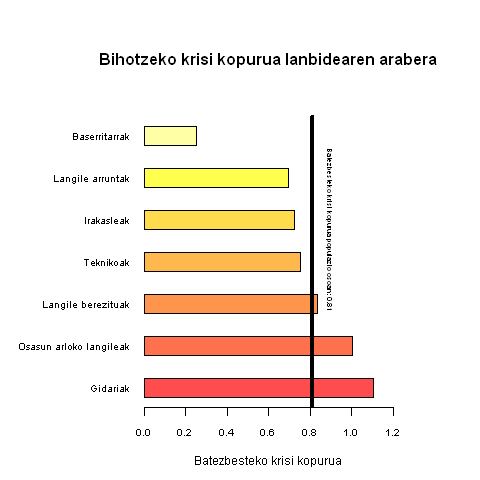
\includegraphics[scale=0.6]{figura2.png}}
\end{figure}

\chapter{Design}

\section{Europe}
\lipsum[1-2]
\begin{figure}[H]
	\ffigbox[\FBwidth]
	{\caption[Estructura de la población mundial]{Estructura de la población mundial \cite{schmitt}}}
	{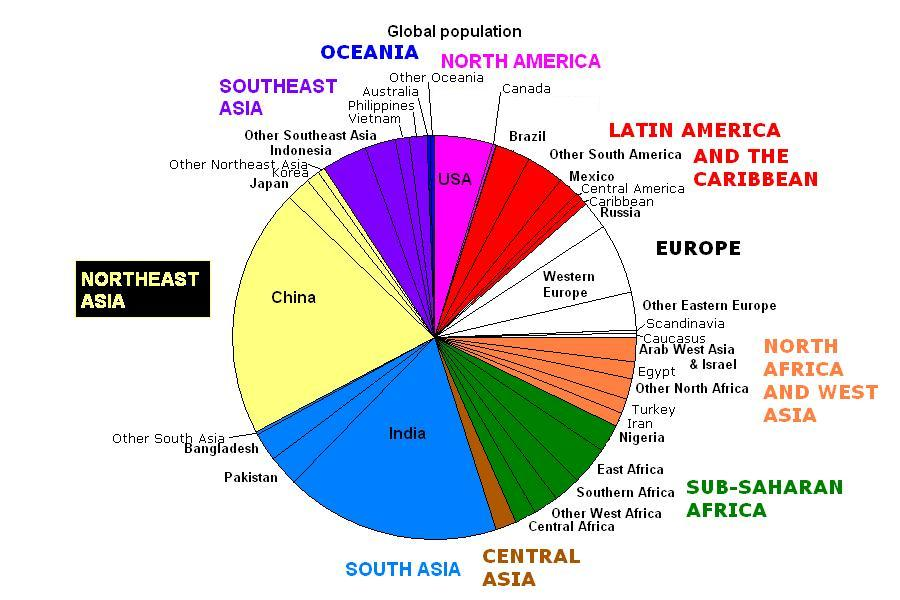
\includegraphics[scale=0.6]{figura3.jpg}}
\end{figure}
\lipsum[39]

\begin{table}[H]
	\ttabbox[\FBwidth]
	{\caption{Lorem ipsum}}
	{\begin{tabular}{|c|P{1.5cm}|c|P{1.5cm}|P{2cm}|c|P{1.5cm}|P{2cm}|}
		\hline
		\multicolumn{2}{|c|}{\textbf{I}} & \multicolumn{2}{c|}{\textbf{II}} & \multicolumn{3}{c|}{\textbf{III}} & \textbf{IV} \\
		\hline
		x & y & x & y & x & y & x & y \\
		\hline
		10.0 & 8.04 & 10.0 & 9.14 & 10.0 & 7.46 & 8.0 & 6.58 \\
		\hline
		8.0 & 6.95 & 8.0 & 8.14 & 8.0 & 6.77 & 8.0 & 5.76 \\
		\hline
		13.0 & 7.58 & 13.0 & 8.74 & 13.0 & 12.74 & 8.0 & 7.71 \\
		\hline
		9.0 & 8.81 & 9.0 & 8.77 & 9.0 & 7.11 & 8.0 & 8.84 \\
		\hline
		11.0 & 8.33 & 11.0 & 9.26 & 11.0 & 7.81 & 8.0 & 8.47 \\
		\hline
		14.0 & 9.96 & 14.0 & 8.10 & 14.0 & 8.84 & 8.0 & 7.04 \\
		\hline
		6.0 & 7.24 & 6.0 & 6.13 & 6.0 & 6.08 & 8.0 & 5.25 \\
		\hline
		4.0 & 4.26 & 4.0 & 3.10 & 4.0 & 5.39 & 19.0 & 12.50 \\
		\hline
		12.0 & 10.84 & 12.0 & 9.13 & 12.0 & 8.15 & 8.0 & 5.56 \\
		\hline
		7.0 & 4.82 & 7.0 & 7.26 & 7.0 & 6.42 & 8.0 & 7.91 \\
		\hline
		5.0 & 5.68 & 5.0 & 4.74 & 5.0 & 5.73 & 8.0 & 6.89 \\
		\hline
		\multicolumn{8}{|l|}{Fuente BOE} \\
		\hline
	\end{tabular}}
\end{table}

\begin{table}[H]
	\ttabbox[\FBwidth]
	{\caption{Lorem ipsum}}
	{\begin{tabular}{|c|P{1.5cm}|c|P{1.5cm}|P{2cm}|c|P{1.5cm}|P{2cm}|}
			\hline
			\multicolumn{2}{|c|}{\textbf{I}} & \multicolumn{2}{c|}{\textbf{II}} & \multicolumn{3}{c|}{\textbf{III}} & \textbf{IV} \\
			\hline
			x & y & x & y & x & y & x & y \\
			\hline
			10.0 & 8.04 & 10.0 & 9.14 & 10.0 & 7.46 & 8.0 & 6.58 \\
			\hline
			8.0 & 6.95 & 8.0 & 8.14 & 8.0 & 6.77 & 8.0 & 5.76 \\
			\hline
			13.0 & 7.58 & 13.0 & 8.74 & 13.0 & 12.74 & 8.0 & 7.71 \\
			\hline
			9.0 & 8.81 & 9.0 & 8.77 & 9.0 & 7.11 & 8.0 & 8.84 \\
			\hline
			11.0 & 8.33 & 11.0 & 9.26 & 11.0 & 7.81 & 8.0 & 8.47 \\
			\hline
			14.0 & 9.96 & 14.0 & 8.10 & 14.0 & 8.84 & 8.0 & 7.04 \\
			\hline
			6.0 & 7.24 & 6.0 & 6.13 & 6.0 & 6.08 & 8.0 & 5.25 \\
			\hline
			4.0 & 4.26 & 4.0 & 3.10 & 4.0 & 5.39 & 19.0 & 12.50 \\
			\hline
			12.0 & 10.84 & 12.0 & 9.13 & 12.0 & 8.15 & 8.0 & 5.56 \\
			\hline
			7.0 & 4.82 & 7.0 & 7.26 & 7.0 & 6.42 & 8.0 & 7.91 \\
			\hline
			5.0 & 5.68 & 5.0 & 4.74 & 5.0 & 5.73 & 8.0 & 6.89 \\
			\hline
			\multicolumn{8}{|l|}{Fuente BOE} \\
			\hline
	\end{tabular}}
\end{table}

\begin{figure}[H]
	\ffigbox[\FBwidth]
	{\caption[Registro de desplazamiento de 5 bits, con entrada paralelo y salida serie]{Registro de desplazamiento de 5 bits, con entrada paralelo y salida serie \cite{purewal}}}
	{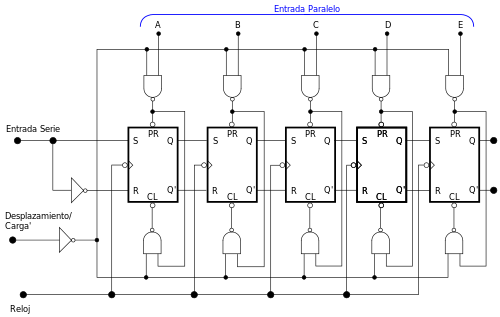
\includegraphics[scale=0.6]{figura4.png}}
\end{figure}

\lipsum[98]


\section{America}
\lipsum[30-32]

\begin{figure}[H]
	\ffigbox[\FBwidth]
	{\caption[Diagrama de lenguas del mundo]{Diagrama de lenguas del mundo \cite{mcfarland}}}
	{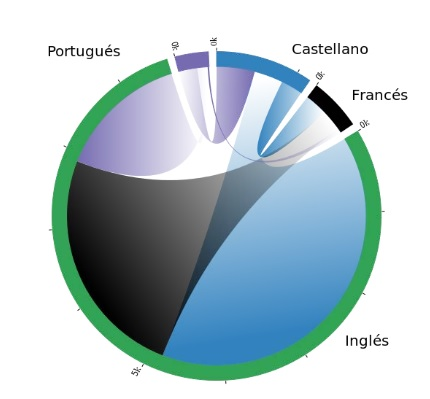
\includegraphics{figura5.jpg}}
\end{figure}

\lipsum[40-41]

\begin{figure}[H]
	\ffigbox[\FBwidth]
	{\caption[Diagrama de flujo de redes]{Diagrama de flujo de redes \cite{mcfarland}}}
	{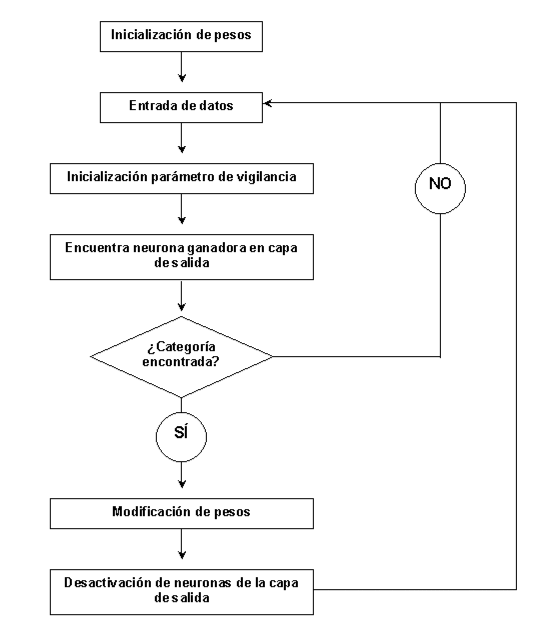
\includegraphics{figura6.png}}
\end{figure}

\lipsum[50-51]

\begin{lstlisting}[language=C++]
#include<iostream>
#include<string>
using namespace std;
int main()
{
string apno;
float hrtr,tahr,subt,boni,tota;
cout<<"Calculos de pagos\n\n";
cout<<"Nombres:\t";cin>>apno;
cout<<endl<<endl<<"Horas Trabajadas:\t";cin>>hrtr;
if (hrtr<=0)
cout<<"No trabajo nada"<<endl;else
{cout<<"Tarifa por hora:\t";cin>>tahr;
subt=hrtr*tahr;
if(hrtr>192)
boni=subt*0.05;
else
boni=subt*0.03;
tota=subt+boni;
cout<<"El sub total es:\t"<<subt<<endl;
cout<<"La bonifiacion es:\t"<<boni<<endl;
cout<<"El total a pagar es:\t"<<tota<<endl<<endl;
}cin.ignore(); return 0;
}
\end{lstlisting}

\lipsum[51]

\chapter{Planning and Budgeting}

\lipsum[103]

\begin{table} [h]
	\ttabbox[\FBwidth]
	{\caption{Presupuestos A y B}}
	{\begin{tabular}{|p{3cm}|p{3cm}|p{3cm}|p{3cm}|}
		\hline
		\rowcolor{gray75}	
		Nombre & Apellido & Presupuesto A & Presupuesto B \\
		\hline
		Ada & Stevens & 2631549 & 705310 \\
		\hline
		Alina & Moore & 7614534 & 8431172 \\
		\hline
		Miley & Phillips & 3290536 & 7275035\\
		\hline
		Samantha & Ryan & 9972831 & 5322273 \\
		\hline
		Penelope & Andrews & 3314907 & 914859\\
		\hline
		Thomas & Alexander & 4111758 & 3088142 \\
		\hline
		Reid & Sullivan & 5552792 & 1248356 \\
		\hline
		Kirsten & Cameron & 2780452 & 9393353 \\
		\hline
		Aiden & Payne & 3982404 & 4985431 \\
		\hline
		Vincent & Ross & 4316417 & 6869331\\
		\hline
		\multicolumn{4}{|l|}{Fuente RANDAT} \\
		\hline
	\end{tabular}}
\end{table}

\lipsum[5-7]	

\begin{table} [h]
	\ttabbox[\FBwidth]
	{\caption{Ítems por empleado}}
	{\begin{tabular}{|p{1.75cm}|p{2cm}|p{2.5cm}|p{1.5cm}|p{2.5cm}|p{1.5cm}|}
		\hline
		\rowcolor{gray75}	
		Nombre & Apellido & Teléfono & Años & Salario & Ítems \\
		\hline 
		Dominik & Perkins & 324-7244-52 & 24 & 189491 & 2 \\
		\hline
		Alissa & Wright & 754-9052-35 & 9 & 74458 & 2 \\
		\hline
		Derek & Hunt & 400-4833-00 & 27 & 100900 & 3 \\
		\hline
		Dominik & Payne & 659-3850-02 & 4 & 89965 & 3 \\
		\hline
		Rafael & Henderson & 856-0458-34 & 2 & 148677 & 2 \\
		\hline
		Violet & Wells & 212-0225-15 & 22 & 168367 & 0\\
		\hline
		Adele & Nelson & 130-5688-00 & 15 & 176676 & 1 \\
		\hline
		Cherry & Lloyd & 887-2631-74 & 27 & 192515 & 5 \\
		\hline
		Aston & Andrews & 108-8120-94 & 14 & 179556 & 3 \\
		\hline
		\multicolumn{6}{|l|}{Fuente INE} \\
		\hline
	\end{tabular}}
\end{table}

\lipsum[6]

\chapter{Conclusions}

\section{Objectives met}
\lipsum[15-16]

\section{Future lines of work}
\lipsum[12-13]

	

%----------
%	BIBLIOGRAFÍA
%----------	

\nocite{*} % Si quieres que aparezcan en la bibliografía todos los documentos que la componen (también los que no estén citados en el texto) descomenta está lína

\clearpage
\addcontentsline{toc}{chapter}{Bibliography}

\printbibliography



%----------
%	ANEXOS
%----------	

% Si tu trabajo incluye anexos, puedes descomentar las siguientes líneas
\chapter* {Annex A. Glosary}
\pagenumbering{gobble} % Las páginas de los anexos no se numeran

\begin{tabbing}	
EASE \quad\=	European Association of Science Editors \\
ECTS \>	Sistema Europeo de Transferencia de Créditos \\
EEES \> Espacio Europeo de Educación Superior \\
TFG	\>	Trabajo de Fin de Grado \\
TFM	\>	Trabajo de Fin de Máster \\
UC3M \>	Universidad Carlos III de Madrid 
\end{tabbing}


\end{document}